\documentclass[ucs,11pt]{beamer}

\usepackage[utf8]{inputenc}
\usepackage[english]{babel}
\usepackage{graphicx}
\usepackage{amsmath}


% Bla bla bla
% Das Template hab ich ein bisschen anpassen muessen, da pgfdeclareimage usw. irgendwie
% nicht mehr funktionieren wollte. Moeglicherweise aufgrund einer neuen Version o.Ae.
% So gehts aber auch.


% Template for talks using the Corporate Design of the Freie Universitaet
%   Berlin, created following the guidelines on www.fu-berlin.de/cd by
%   Tobias G. Pfeiffer, <tobias.pfeiffer@math.fu-berlin.de>
% This file can be redistributed and/or modified in any way you like.
%   If you feel you have done significant improvements to this template,
%   please consider providing your modified version to
%   https://www.mi.fu-berlin.de/w/Mi/BeamerTemplateCorporateDesign

% NOTE: Removed pgf because it didn't work for me.

%%% FU logo
% small version for upper right corner of normal pages
%\pgfdeclareimage[height=0.9cm]{university-logo}{FULogo_RGB}
%\logo{\pgfuseimage{university-logo}}
% large version for upper right corner of title page
%\pgfdeclareimage[height=1.085cm]{big-university-logo}{FULogo_RGB}
%\newcommand{\titleimage}[1]{\pgfdeclareimage[height=2.92cm]{title-image}{#1}}
%\titlegraphic{\pgfuseimage{title-image}}
%%% end FU logo

\logo{
\includegraphics[height=0.9cm]{FULogo_RGB.png}}
\newcommand{\titleimage}[1]{\titlegraphic{\includegraphics[height=2.92cm]{#1}}}

% NOTE: 1cm = 0.393 in = 28.346 pt;    1 pt = 1/72 in = 0.0352 cm
\setbeamersize{text margin right=2.5mm, text margin left=7.5mm}  % text margin

% colors to be used
\definecolor{text-grey}{rgb}{0.45, 0.45, 0.45} % grey text on white background
\definecolor{bg-grey}{rgb}{0.66, 0.65, 0.60} % grey background (for white text)
\definecolor{fu-blue}{RGB}{0, 51, 102} % blue text
\definecolor{fu-green}{RGB}{153, 204, 0} % green text
\definecolor{fu-red}{RGB}{204, 0, 0} % red text (used by \alert)

% switch off the sidebars
% TODO: loading \useoutertheme{sidebar} (which is maybe wanted) also inserts
%   a sidebar on title page (unwanted), also indents the page title (unwanted?),
%   and duplicates the navigation symbols (unwanted)
\setbeamersize{sidebar width left=0cm, sidebar width right=0mm}
\setbeamertemplate{sidebar right}{}
\setbeamertemplate{sidebar left}{}
%    XOR
% \useoutertheme{sidebar}

% frame title
% is truncated before logo and splits on two lines
% if neccessary (or manually using \\)
\setbeamertemplate{frametitle}{%
    \vskip-30pt \color{text-grey}\large%
    \begin{minipage}[b][23pt]{80.5mm}%
    \flushleft\insertframetitle%
    \end{minipage}%
}

%%% title page
% TODO: get rid of the navigation symbols on the title page.
%   actually, \frame[plain] *should* remove them...
\setbeamertemplate{title page}{
% upper right: FU logo
\vskip2pt\hfill
\includegraphics[height=1.085cm]{FULogo_RGB} \\
\vskip6pt\hskip3pt
% title image of the presentation
\begin{minipage}{11.6cm}
\hspace{-1mm}\inserttitlegraphic
\end{minipage}

% set the title and the author
\vskip14pt
\parbox[top][1.35cm][c]{11cm}{\color{text-grey}\inserttitle \\ \small \insertsubtitle}
\vskip11pt
\parbox[top][1.35cm][c]{11cm}{ \insertinstitute \\[3mm] \insertdate}
}
%%% end title page

%%% colors
\usecolortheme{lily}
\setbeamercolor*{normal text}{fg=black,bg=white}
\setbeamercolor*{alerted text}{fg=fu-red}
\setbeamercolor*{example text}{fg=fu-green}
\setbeamercolor*{structure}{fg=fu-blue}

\setbeamercolor*{block title}{fg=white,bg=black!50}
\setbeamercolor*{block title alerted}{fg=white,bg=black!50}
\setbeamercolor*{block title example}{fg=white,bg=black!50}

\setbeamercolor*{block body}{bg=black!10}
\setbeamercolor*{block body alerted}{bg=black!10}
\setbeamercolor*{block body example}{bg=black!10}

\setbeamercolor{bibliography entry author}{fg=fu-blue}
% TODO: this doesn't work at all:
\setbeamercolor{bibliography entry journal}{fg=text-grey}

\setbeamercolor{item}{fg=fu-blue}
\setbeamercolor{navigation symbols}{fg=text-grey,bg=bg-grey}
%%% end colors

%%% headline
\setbeamertemplate{headline}{
\vskip4pt\hfill\insertlogo\hspace{3.5mm} % logo on the right

\vskip6pt\color{fu-blue}\rule{\textwidth}{0.4pt} % horizontal line
}
%%% end headline

%%% footline
\newcommand{\footlinetext}{\insertshortinstitute, \insertshorttitle, \insertshortdate}
\setbeamertemplate{footline}{
\vskip5pt\color{fu-blue}\rule{\textwidth}{0.4pt}\\ % horizontal line
\vskip2pt
\makebox[123mm]{\hspace{7.5mm}
\color{fu-blue}\footlinetext
\hfill \raisebox{-1pt}{\usebeamertemplate***{navigation symbols}}
\hfill \insertframenumber}
\vskip4pt
}
%%% end footline

\beamersetuncovermixins{\opaqueness<1>{25}}{\opaqueness<2->{15}}

\titleimage{fu_500.jpg}

\title[Punktgruppen]{Visualisierung der 3D/4D Punktgruppen}
\subtitle{Abschlusspräsentation}
\institute[FU Berlin]{Freie Universität Berlin}
\date[30.1.2014]{30. Januar 2014}

\begin{document}

\begin{frame}[plain]
	\titlepage
\end{frame}

\begin{frame}{Aufgabe}
	\begin{enumerate}
		\item Modellierung und Darstellung von Symmetrien von 3-dimensionalen Polyedern \pause
		\item und von 4-dimensionalen Polyedern. \pause
		\item Visualisierung als Schlegeldiagramm. \pause
		\item Anzeigen des Fundamentalbereichs.
	\end{enumerate}
\end{frame}


\begin{frame}{Details zu Aufgabe 1 und 2}

\begin{columns}
\begin{column}{.48\textwidth}
\begin{enumerate}
	\item Wählen einer Symmetriegruppe	
 \visible<2->{
	\item Wählen eines Punktes im Fundamentalbereich \\
	      \vspace{0.5cm}
	      \emph{Abbilden des Punktes unter der Symmetriegruppe}
}
 \visible<3->{
	\item Darstellung als Schlegeldiagramm 
}
	\end{enumerate}
\end{column}%
\hfill%
\begin{column}{.48\textwidth}
\only<1>{
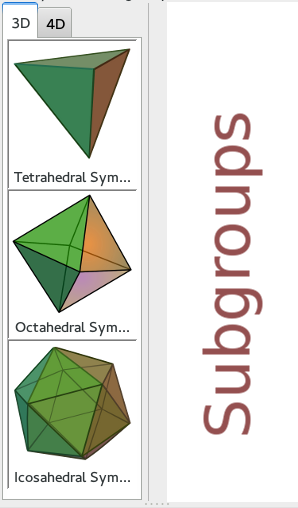
\includegraphics[width=0.5\textwidth]{symmetryChoose.png}
}
\only<2>{
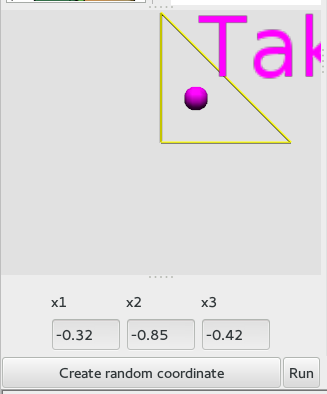
\includegraphics[width=0.8\textwidth]{pointPicker.png}
}
\only<3>{
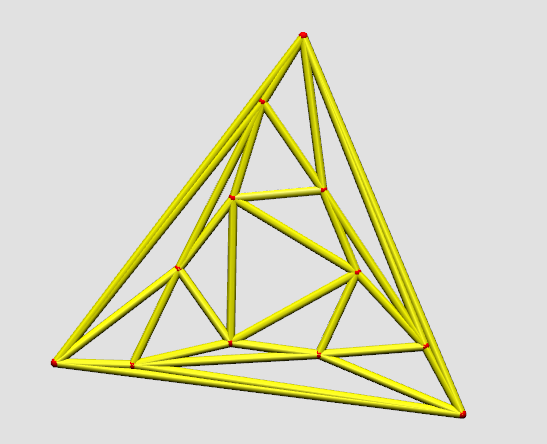
\includegraphics[width=1\textwidth]{schlegelView.png}
}
\end{column}%
\end{columns}	
\end{frame}

\begin{frame}{Meilensteine}
	\begin{enumerate}
		\item Schnittstelle zwischen Java und Polymake, Architekturentwurf \& mathematische Grundlagen erarbeiten 
		\item 3D-Symmetrien umsetzen
		\item grafische Darstellung erarbeiten
		\item 4D-Symmetrien umsetzen
	\end{enumerate}
\end{frame}

\begin{frame}{Umsetzung der Meilensteine}
\begin{enumerate}
		\item Schnittstelle zwischen Java und Polymake, Architekturentwurf \& mathematische Grundlagen erarbeiten \pause 
\visible<3->{ \checkmark }
\visible<2>{
			\begin{itemize}
				\item Schnittstelle über TCP erstellt
				\item Grobes Verständnis der Quaternionen 
			\end{itemize}
}
		\item 3D-Fall lösen \pause \visible<5->{ \checkmark }
\visible<4>{			
			\begin{itemize}
				\item Repräsentation der Quaternionen und Berechnung der Punkmenge in Java
				\item Berechnung der konvexe Hülle \& des Schlegeldiagramms in Polymake 
				\item Symmetriegruppen Tetraeder, Oktaeder \& Ikosaeder hartcodiert
				\item Fundamentalbereich in Java und Polymake %Extra Folie
			\end{itemize}
}
		\item grafische Darstellung \pause \visible<7->{ \checkmark }
\visible<6>{
			\begin{itemize}
				\item Keine Verwendung von JavaView % Warum? Weil nicht opensource und keine Integration in JFrame einfach möglich.
				\item Alternative: JReality %Extra Folie
				\item Einbindung in JFrame %Bild?!
			\end{itemize}
}
		\item 4D-Fall lösen \pause
\visible<8>{
			\begin{itemize}
				\item Hauptproblem: Erstellung der Symmetriegruppen
				\item Elemente einer Symmetriegruppe nicht dokumentiert
				\item Kreuzprodukt zweier 3D-Symmetriegruppen nicht dokumentiert
			\end{itemize}
}
	\end{enumerate}
\end{frame}

\begin{frame}{Fundamentalbereich}
TODO
\end{frame}

\begin{frame}{Organisation}
		\begin{itemize}
			\item Git, Mailingliste, SplinePad \pause
			\item wöchentliches Meeting \pause
				\begin{itemize}
					\item Wer hat was getan?
					\item Diskussion über aktuelle Probleme
					\item Aufgabenverteilung für die nächste Woche
				\end{itemize} \pause
			\item T$^\bigstar$-Modell \pause
			\item Java, Eclipse, polymake, JReality \pause
			\item Coding Style, BSD Lizenz
		\end{itemize}
\end{frame}

\begin{frame}{JReality}

\begin{columns}
	\begin{column}{.48\textwidth}
		\begin{itemize}
			\item Opensource Java Bibliothek für 3D Anwendungen
			\item TU Berlin http://www3.math.tu-berlin.de/jreality/
			\item OpenGL
		\end{itemize}
	\end{column}%
	\hfill%
	\begin{column}{.48\textwidth}
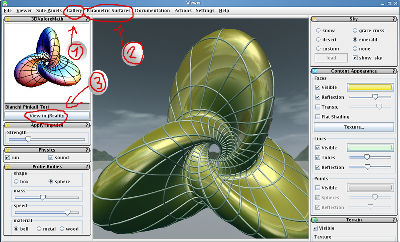
\includegraphics[width=1\textwidth]{jRealityBla.png}
	\end{column}%
\end{columns}
\end{frame}


\begin{frame}[t]{Architektur}
\vspace{1.5cm}
	\begin{itemize}
		\item Eventbasierte Stern-Architektur \pause
		\item Lose Kopplung zwischen den Komponenten \pause
		\item Asynchrone Brücken zwischen Java und Polymke \pause
		\item Berechnungsanfragen als Perl-Programme \pause
		\item Symmetriegruppen als einzelne Klassen
	\end{itemize}
\vspace{1cm}
\only<5->{\emph{Siehe folgendes Bild}}
\end{frame}

\begin{frame}{Architektur}
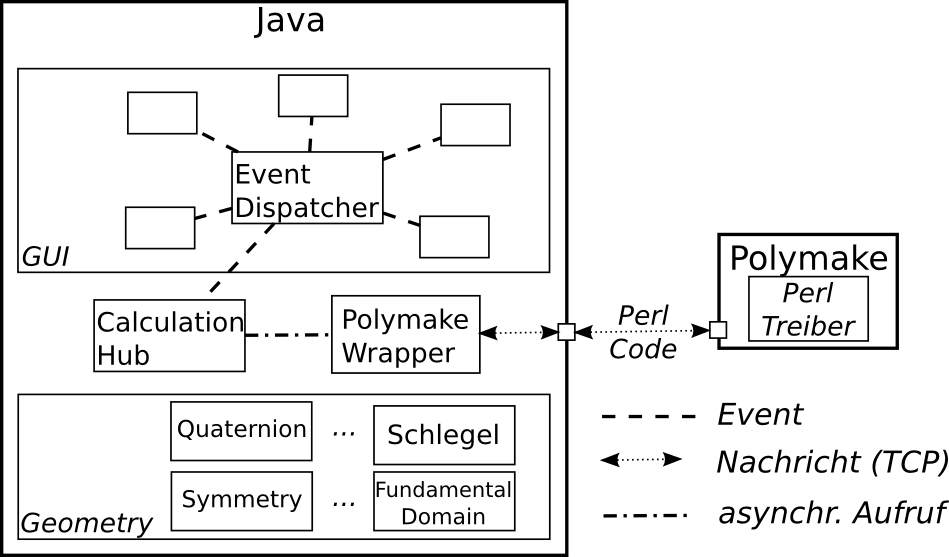
\includegraphics[width=1\textwidth]{architecture.png}
\end{frame}

\begin{frame}{Demo}
\huge{Siehe: Live-Demo}
\end{frame}

\begin{frame}{Zusammenfassung der Funktionen}
	\begin{itemize}
		\item Auswahl 3D/4D \pause
		\item Symmetriegruppen: Tetraeder, Oktaeder \& Ikosaeder \pause
		\item Punktwahl im Raum, Eingabe oder zufällig \pause
		\item Darstellung des Fundamentalbereichs \pause
		\item Darstellung der Punktgruppe als Schlegeldiagramm \pause
		\item Logbuch 	
	\end{itemize}
\end{frame}

\begin{frame}{Lesson Learned}
	\begin{itemize}
		\item Für Projekt und Teilnehmeranzahl gutes Prozessmodell \pause
		\item Wöchentliches Meeting sinnvoll \pause
		\item Protokoll hilfreich zur Erinnerung und Fokussierung der Besprechung (Spline-Pad) \pause
		\item Persönliche Kommunikation notwendig \pause
		\item Meist guter Einsatz von Git \pause
		\item Verwendung von Fremdsoftware aufwendig \pause
		\item Softwareprojekte als Blockkurs sind angenehmer \pause
	\end{itemize}
\end{frame}

\begin{frame}{Ausblick}
\begin{itemize}
	\item Symmetriegruppen aus Erzeugern generieren
	\item GUI verschönern
	%\item Schnittstelle um Polyeder im 3D-Drucker ausdrucken zu können
	\item Logbucheintragstufe einstellen
	\item Parallelisierung der Anfragen an Polymake
\end{itemize}
\end{frame}


\begin{frame}[t]{Fragen}
\vspace{1cm}
\huge{Vielen Dank für die Aufmerksamkeit!} \\
\vspace{1cm}
\only<2->{\huge{Fragen?}}
\end{frame}
\end{document}
